\documentclass[british,titlepage]{ntnuthesis}

\title{Long-term vessel trajectory inference using Gaussian Processes }
\shorttitle{Gaussian Process Trajectory Inference}
\author{%
Håvard Skåra Mellbye
\vspace{1cm}\\
Supervisor: Edmund Førland Brekke \\ 
Co-supervisor: Trym Tengesdal
}
\shortauthor{Mellbye}
\date{}


\addbibresource{thesis.bib}

\usepackage{tikz}
\usetikzlibrary{bayesnet}
\usepackage{ifthen}
\usepackage[many]{tcolorbox}
\usepackage{todonotes}



% From https://www.overleaf.com/learn/latex/Glossaries

\makeglossaries % Prepare for adding glossary entries



% --------------------
% ----- Acronyms -----
% --------------------

\newacronym{mcmc}{MCMC}{Markov Chain Monte Carlo}
\newacronym{pgm}{PGM}{Probabilistic Graphical Model}
\newacronym{bp}{BP}{Belief Propagation}
\newacronym{dgm}{DGM}{Directed Graphical Models}
\newacronym{mrf}{MRF}{Markov Random Fields}
\newacronym{kl}{KL}{Kullback-Liebler divergence}
\newacronym{pdf}{PDF}{Probability Density Function}
\newacronym{pmf}{PMF}{Probability Mass Function}
\newacronym{vi}{VI}{Variational Inference}
\newacronym{elbo}{ELBO}{Evidence Lower Bound}
\newacronym{hmc}{HMC}{Hamiltonian Monte Carlo}

\newglossaryentry{moralization}
{
    name=moralization,
    description={The process of converting Directed Graphical Models into Markov Random Fields}
}

\newglossaryentry{support}{
    name=support,
    description={The set of possible outcomes/values with a non-zero probability, i.e. all events that can happen. A Gaussian distribution for example have support for $x \in \mathcal{R}$ since it has a non-zero probability, $p(x) > 0$, for all real numbers $x \in \mathcal{R}$.}
} % add glossary and acronym lists before document

\begin{document}
% gives the width of the current document in pts
\chapter*{Abstract}

Autonomous ships depend on situational awareness in order to avoid collisions in a safe and robust manner. By knowing the intention of surrounding vessels, safety margins can be improved by avoiding situations with increased risk. In this thesis, methods for Bayesian Inference will be explored, with the goal of developing a flexible framework for intention modelling. Exact and approximate inference methods are explored. Approximate methods are found to be more flexible, allowing easier incorporation of existing knowledge from domain experts or conventions such as \Gls{colregs}. Methods such as \acrfull{mcmc} and \acrfull{vi} are therefore explored further and compared on an illustrative intention model. The results then find \acrshort{mcmc} to be accurate at the cost of computational complexity. \acrshort{vi} on the other hand, is found to be a lot faster, though much less precise on the illustrative model. 

\tableofcontents
\listoffigures
\listoftables
%\lstlistoflistings


\printglossary[type=\acronymtype] % Print acronyms
\printglossary                    % Print glossary

\chapter{Introduction}

\begin{figure}[h]
    \centering
    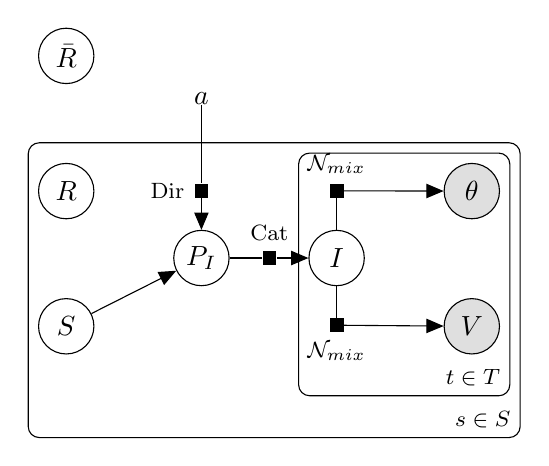
\begin{tikzpicture}
        % NODES
        \node[latent] (I) {$I$};
        \node[obs, right=of I, yshift=0.85cm] (theta) {$\theta$};
        \node[latent, left=of I] (PI){$P_I$};
        \node[obs, below=of theta] (V) {$V$};
        \node[latent, left=of PI, yshift=0.85cm] (R) {$R$};
        \node[latent, above=of R] (RR) {$\bar{R}$};
        \node[latent, below= of R] (S) {$S$};
        
        % FACTORS
        \factor[above=of I] {theta-f}{$\mathcal{N}_{mix}$}{}{};
        \factor[below=of I]{v-f}{below:$\mathcal{N}_{mix}$}{}{};
        \factor[left=of I]{I-f}{Cat}{}{};
        \factor[above=of PI]{PI-f}{left:Dir}{}{};

        \node[const, above=of PI-f] (a) {$a$};
        
        \factoredge {I} {theta-f} {theta};
        \factoredge {I} {v-f} {V};
        \factoredge{PI}{I-f}{I};
        \factoredge{a}{PI-f}{PI};

        \edge{S}{PI};

        \plate {ship}{(I)(theta)(V)}{$t \in T$};
        \plate {}{(I)(theta)(V)(R)(S)(ship)}{$s \in S$};
        
        
    \end{tikzpicture}
\end{figure}

\chapter{AIS}

The \textit{\acrfull{ais}} is a vessel-to-vessel communication system, which allows vessels to share vital information about their current state.

\section{The Dataset}

\begin{figure}[h]
    \centering
    \begin{subfigure}{\textwidth}
        \centering
        \includegraphics{figures/ais_map.pdf}
        \caption{Full dataset. The red areas marks the subset which will be used for testing purposes.}
    \end{subfigure}
    \begin{subfigure}{\textwidth}
        \centering
        \includegraphics{figures/ais_map_zoom.pdf}
        \caption{Zoomed-in version of the subset used in this thesis.}
    \end{subfigure}
    \caption{The available \acrshort{ais} data used in this thesis. }
\end{figure}


\section{From individual samples to trajectories}\label{sec:from_ais_to_traj}
\acrshort{ais} samples with identical MMSI and less than $15$ minutes between subsequent samples are considered part of the same trajectory. The $15$ minute requirement is added to make sure samples before and after docking are considered separate trajectories.


\chapter{Previous Work}\label{chap:prior_work}

There is currently limited work available on using \acrshort{gp}s on \acrshort{ais} data.

\citeauthor{gpanomaly} propose a method for anomaly detection of moving vessels in \cite{gpanomaly}. The approach uses a \acrshort{gp} to learn vessels' normal behavior in an area, which is then used to detect abnormal behavior. The work further addresses the computational challenges when using large datasets and proposes an active learning approach that iteratively adds new training samples to select the optimal training sample. A relatively small sample size is then used to represent the entire dataset. Active learning is computationally feasible by updating the Cholesky decomposition at each step instead of recomputing the entire decomposition. While the approach works well for anomaly detection, it was not intended for predicting future trajectories, only to classify existing trajectories.

\citeauthor{gp_ais_trajectory} address the problem of trajectory uncertainty in \cite{gp_ais_trajectory}. The paper proposes a method for probabilistic trajectory prediction using \acrshort{gp}s, where different distributions describe the lateral and longitudinal directions of the trajectory. The parameters of the distributions are learned offline based on historical \acrshort{ais} data. They are then applied in real-time by adding new observations through a Cholesky update to avoid recomputing the decomposition. The model uses the common \acrshort{rbf} kernel, and the hyperparameters are selected as the median of the maximum likelihood estimates for each unique vessel. The prediction is then conditioned on historical \acrshort{ais} samples for a given vessel.
A case study is performed where the model is trained and tested on three months of \acrshort{ais} data along a smooth traffic lane. The methods yield high prediction accuracy even for long prediction horizons while still applying to real-time applications. Only a highly smooth traffic lane with little curvature is used, and the paper does not mention the performance on curved trajectories. As the model is only conditioned on previous samples of a given vessel, it is unlikely that the model is able to predict upcoming turns. 

There is, however, extensive work on using \acrshort{gp}s for trajectory prediction outside of the maritime field. \citeauthor{vehicle_gp_prediction} \cite{vehicle_gp_prediction} utilizes \acrshort{gp}s for long-term trajectory prediction for collision avoidance in a connected vehicle environment. The vehicles are assumed to share position through vehicle-to-vehicle communication, somewhat in a similar fashion to \acrshort{ais} for maritime vessels. The paper uses a \acrshort{gp} to learn a motion model from historical data, mapping a vehicle's current position to a trajectory derivative. The historical data is clustered into a finite number of clusters, where the trajectories in each cluster are assumed to have similar properties. The paper utilizes K-means clustering \cite{murphy} to group trajectories based on the first and last position of a trajectory. For each cluster, independent \acrshort{gp}s are then fitted for each of the two coordinate axes, using independent \acrshort{rbf} kernels and zero mean priors. While this method should be applicable to \acrshort{ais} data, there are a few key distinctions to keep in mind:
\begin{enumerate}
    \item In this paper, the trajectory derivatives are calculated using finite difference with a sampling interval of $0.1$ seconds. The typical sampling interval for \acrshort{ais} data is in the range of minutes, so relying on numerical derivatives might be challenging.
    \item The vehicles trajectories are from an intersection, and the roads constrain the vehicles' behavior. There is, therefore, only a finite number of route options a vehicle may take.
\end{enumerate}

A similar approach is used by \citeauthor{pedestrian} \cite{pedestrian} to predict the trajectory of pedestrians tracked using computer vision. The paper also learns a dynamical model using \acrshort{gp}s but utilizes a Bayes Filter framework proposed by \citeauthor{gpekf} in \cite{gpekf} to simulate the trajectories. Two different approaches were used:
\begin{enumerate}
    \item By assuming $p(\boldsymbol{x})$ is always uni-modal and Gaussian, the GP-EKF introduced in \cite{gpekf} was used to simulate the trajectory for multiple timesteps, using the dynamical \acrshort{gp} model as the prediction model. The GP-EKF is based on the Extended Kalman Filter, where the prediction model is learned from data using a \acrshort{gp}. This formulation is unable to express multimodal uncertainty.
    \item To retain the inherent multimodality, a sequential Monte-Carlo approach (i.e., the prediction step of a particle filter) was used to keep track of multiple modes (i.e., branching trajectories) at the cost of computational complexity.  
\end{enumerate}


\subsection{Clustering-based method}
A common approach for trajectory prediction using \acrshort{ais} is based on clustering methods. This approach can typically be divided into four steps \cite{dalsnes-hexeberg}:

\begin{enumerate}
    \item Cluster trajectories based on historical data
    \item Classify new target vessels into the appropriate cluster
    \item Generate a representative trajectory the given cluster
    \item Predict the movement using the representative trajectory.
\end{enumerate}

Examples of this approach can be found in\cite{palotta}, \cite{mazzarella} and \cite{mazzarella2}. 


Traditional clustering methods, such as k-means or DBSCAN, tend to focus on clustering point values. In the context of trajectory prediction, the trajectories would then be clustered as a whole. The trajectory clustering algorithm TRACLUS was therefore introduced by \cite{traclus} where it was applied to hurricane trajectory and animal movement data. The key observation was that trajectories might have portions that share common behavior, while the entire trajectory might still differ. TRACLUS allows clustering trajectories based on common sub-trajectories and works by partitioning the trajectories into smaller line segments and then groups similar segments into clusters. 

\section{Data Driven Approches}
\citeauthor{hexeberg} introduced the \textit{Single Point Neighborhood Search} (SPNS), a purely data-driven approach, in \cite{Hexeberg2017AISbasedVT}. It deviates from the clustering-based methods as it estimates the future course and speed at each prediction time based on historical \acrshort{ais} data. \todo[]{Finish writing about Simen And Bjørnar's work} 

\chapter{Neccessary Theoretical Background}

\section{Useful Results From Probability Theory}


 
\subsection{Conditional Probabilities}
The conditional probability $p(A | B)$ is the probability of $A$ occurring, given that we know $B$ has occured. 
\begin{equation}
    p(A | B) = \frac{p(A, B)}{p(B)}
\end{equation}



\section{Bayesian Statistics}

\section{Stochastic Modelling}

\section{Probabilistic Graphical Models}

\section{Belief Propagation}

\section{Markov Chains}


\chapter{Learning trajectories directly from data}
As a first attempt on using \acrshort{gp}s for trajectory prediction, a direct approach was attempted. The idea was to use a \acrshort{gp} to model a function $f: \mathcal{R}^5 \to \mathcal{R}^2$, mapping a ships current position $\boldsymbol{p}_t$, \acrshort{cog} $\psi_t$ and \acrshort{sog} $v_t$ to a position at time $t+\tau$. The method is formulated in mathematical terms in \cref{eq:gp_direct}. 

\begin{subequations}\label{eq:gp_direct}
\begin{align}
    \boldsymbol{f}(\boldsymbol{x}) &= \boldsymbol{p}_{\tau} \label{eq:gp_direct_f}, \quad \boldsymbol{x} = \begin{bmatrix} \boldsymbol{p}_0 & \psi_0 & v_0 & \tau\end{bmatrix}\\
    \boldsymbol{f}(\boldsymbol{x}) &\sim \text{GP}(\boldsymbol{m}(\boldsymbol{x}), K(\boldsymbol{x}, \boldsymbol{x}))\label{eq:gp_direct_f_dist}
\end{align} 
\end{subequations}

The model could then be queried about likely future positions by evaluating $\boldsymbol{f}$ with the desired initial conditions and time horizon. 

The conceptual benefits of this formulation include:
\begin{description}
    \item[Continuous formulation] The model directly models the position at any time $t+\tau$ and does not require discretization. 
    \item[Conceptually easy] This formulation directly expresses the unknown trajectory, making it easy to reason about conceptually.
    \item[Simple Problem formulation] The model requires few components.
    \item[Easy incorporation of available AIS data] The reported \acrshort{cog} and \acrshort{sog} can easily be incorporated into the similarity measure, utilizing more of the available data.
\end{description}

However, this formulation was impractical to work with and was abandoned after several attempts to get it to work. The attempted method and the issues which followed are discussed in this chapter.


\section{Implementation}
A large number of input dimensions pose a challenge as it requires large amounts of data, which is infeasible using the exact \acrshort{gp}. Two different approximations were attempted.

\begin{enumerate}
    \item Selecting only a subset of the data which is relevant for a given prediction. Based on the initial conditions in $\boldsymbol{x}$, a subset of representative trajectories can be selected and used for training. The exact \acrshort{gp} formulation in \cref{alg:gp_prediction} can then be used, though it requires both hyperparameter tuning and recalculating Cholesky decomposition $L$ for each query input $x$.
    \item Approximating the \acrshort{gp} using the \acrshort{svgp}, the entire dataset can be used at the cost of increased model complexity. It is also an approximation method, so there are a few tradeoffs when using \acrshort{svgp}. The benefit is that a \acrshort{gp} can be trained once for a large area and be used for multiple predictions.
\end{enumerate}

\subsection{Excact GP with a subset of data}
When making a prediction, only a subset of the \acrshort{ais} data is relevant for any given query. Trajectories with very different initial conditions than the query input should be safe to ignore, leaving only a subset of relevant trajectories to use for training. This way, we can still use the exact \acrshort{gp} formulation and avoid the additional complexity of \acrshort{gp} approximations. The following requirements need to be satisfied for the trajectories used to train the \acrshort{gp}:
\begin{enumerate}
    \item The initial position of the trajectory must be close to the queried position $\boldsymbol{p}_0$. In this thesis, a cutoff was used at $500$ meters from $\boldsymbol{p}_0$.
    \item The initial \acrshort{cog} must be close to the queried heading $\mathcal{X}_0$. A cutoff at $\pm 10^\circ$ for the \acrshort{cog} was used in this thesis.
    \item The initial \acrshort{sog} must be close to the queried velocity $v_0$. A cutoff at $\pm 5 \text{m/s}$ for the \acrshort{sog} was used in this thesis.
\end{enumerate} 

\subsection{Sparse Variational Gaussian Process}
While filtering the data before making a prediction works well for isolated cases, it does not scale well. The model needs to be retrained for each query, which results in a significant performance penalty in practical applications. As an alternative, we can attempt to use the \acrshort{svgp} instead to train a single \acrshort{gp} which can be used for any queries in an area. The training time will be a lot longer but can be performed in advance. 

\section{Choice of kernels}

We attempted multiple types of kernels. 

\section{Implementation}
The model is implemented in \textit{GPFlow} \cite{GPflow2017}, a \acrshort{gp} framework built on the well-known \textit{tensorflow} \cite{tensorflow2015-whitepaper} library. GPFlow has several implementations of \acrshort{gp}s, including both excact implementation and \acrshort{svgp} we have discussed earlier. We will here utilize the \acrshort{svgp} implementation to learn a sparse approximation of \cref{eq:gp_direct} direcly from all available data. 

For optimization, the stochastic gradient optimizer \textit{ADAM} should be familiar for anyone working with Neural Networks. With only a few lines of code, the \acrshort{elbo} can be optimized to get a variational approximation of the true posterior distribution.

\section{Results}

In practice, this formulation turned out to be challenging to work with, primarily due to the increased complexity of \acrshort{svgp} and a large number of input dimensions.

\subsection{Complexity}
Building the model using \acrshort{svgp} turned out to be challenging. While the model sometimes was able to achieve reasonable \acrshort{mse} given enough training iterations, the trajectories were by visual inspection found to be unrealistic. The high complexity of the model made it challenging to pinpoint the underlying cause of prediction errors. The benefit of \acrshort{gp}s interpretability is lost when using these approximate methods.

\subsection{Optimization}
The optimization would often result in unrealistic hyperparameters, such as prioritizing \acrshort{cog} and \acrshort{sog} over the position. This would yield predictions where the initial position was far away from the queried position. This problem could potentially be fixed by specifying priors for the hyperparameters, but this would also further increase the complexity. 

Optimizing both the hyperparameters and the inducing variables was extremely slow and required hours to get good results. Due to the high number of input dimensions, a large number of inducing variables were required to get a good approximation. 





\chapter{Non-parametric dynamic system using AIS tracking data}
One of the significant issues with the direct approach is the unimodal assumption of using a \acrshort{gp}. It works well as long as vessels agree on a specific trajectory but fails as soon as there are multiple branching trajectories.

In \cite{pedestrian}, a \acrshort{gp} was used to model the trajectory patterns of pedestrians tracked using computer vision. Rather than directly describing trajectories, the paper proposed to simulate trajectories from a non-parametric dynamical model $\Delta\boldsymbol{x}_{t+1} = \vec{f}(\boldsymbol{x}_t)$ where the increments are expressed using a \acrshort{gp}. The trajectories were then simulated using two different approaches:
\begin{enumerate}
    \item By assuming $p(\boldsymbol{x})$ is always uni-modal and Gaussian, the GP-EKF introduced in \cite{gpekf} was used to simulate the trajectory for multiple timesteps, using the dynamical \acrshort{gp} model as the prediction model. This formulation is unable to express multimodal uncertainty.
    \item To retain the inherent multimodality, a sequential Monte-Carlo approach (i.e., the prediction step of a particle filter) was used to keep track of multiple modes (i.e., branching trajectories) at the cost of computational complexity.
\end{enumerate}

In this section, a similar method is proposed for long-term vessel prediction. The vessel trajectory $\boldsymbol{\mathcal{T}}$ can be expressed using the dynamical system
\begin{subequations}
    \begin{align}
        \boldsymbol{x}_{t+1} & = \boldsymbol{x}_t + \vec{f}(\boldsymbol{x}_t)                              \\
        \mathcal{T}_t        & = \boldsymbol{x}_t + \epsilon, \quad \epsilon \sim \mathcal{N}(0, \sigma^2)
    \end{align}
\end{subequations}
The function $\vec{f}(\cdot): \mathcal{R}^2 \to \mathcal{R}^2$ denotes the vector field describing the expected velocity. In the case of long-term prediction, the dynamics $\vec{f}(\cdot)$ is unknown and is unlikely to be stationary. Instead of using the usual parametric approaches to ODE models, the goal of this chapter is to use a \acrshort{gp} to create a non-parametric representation of the dynamics $\vec{f}(\cdot)$ by learning from historical trajectories of other vessels. This way, arbitrary complex dynamics can be learned without being limited by parametrization.

\begin{equation}\label{eq:gp_vec_field}
    \vec{f}(\boldsymbol{x}) = \begin{bmatrix} f_x (\boldsymbol{x})\\ f_y (\boldsymbol{x})\end{bmatrix} \sim \text{GP} \big(\begin{bmatrix} m_x(\boldsymbol{x})\\m_y(\boldsymbol{x})\end{bmatrix}, \ \begin{bmatrix}
            K_{xx}(\boldsymbol{x}, \boldsymbol{x}') & K_{xy}(\boldsymbol{x}, \boldsymbol{x}') \\ K_{xy}(\boldsymbol{x}, \boldsymbol{x}')^\intercal & K_{yy}(\boldsymbol{x}, \boldsymbol{x}')
        \end{bmatrix}\big)
\end{equation}

The benefits of this formulation include:
\begin{description}
    \item[Easy incorporation of existing data] The model can easily be trained on partial data. Only the gradients of any historical trajectories are really needed.
    \item[Few constraining assumptions] The dynamical model is not constrained by any specific parametrization while still allows prior knowledge such as smoothness to be incorporated into the model.
    \item[Branching trajectories] The dynamical formulation only assumes Gaussian increments, while the full trajectory may still be multimodal. Though not analytically tractable, the multimodal trajectory can be found using sampling-based methods.
\end{description}

However, the major downside is that the model only learns gradients from data and relies heavily on numerical simulations to get the desired trajectories.

The model could further be improved by clustering the samples based on similar behavior for different ships, such as similar initial course and velocity. Separate \acrshort{gp}s could then be trained on the different subsets of data.

\section{Simulating trajectories using the Gaussian Process Extended Kalman Filter}

\subsection{EKF trajectory prediction}
Once the dynamics $\vec{f}_*$ is conditioned on data, it can be used to predict trajectories using the prediction procedure used by \textit{\acrfull{ekf}}. The combination of \acrshort{gp}s and \acrshort{ekf} was proposed by \cite{gpekf} and is summarized here. The reader is assumed to be already familiar with the Kalman filter and, by extension, the \acrshort{ekf}.

During the prediction procedure, the state is updated incrementally by adding $\vec{f}$ to the current state, i.e. the \acrshort{ekf} prediction model, $g(\boldsymbol{x})$, is given by \cref{eq:gp_ekf_prediction}.

\begin{equation}\label{eq:gp_ekf_prediction}
    \hat{\boldsymbol{x}}_{t} = \boldsymbol{g}(\boldsymbol{x}_{t-1}) = \boldsymbol{x}_{t-1} + \vec{f}(\boldsymbol{x}_{t-1})
\end{equation}

Due to the potentially non-linear dynamics of $\vec{f}$, which implies non-linearity in $\boldsymbol{g}(\cdot)$, we need to linearize the prediction in order to propagate the state uncertianty $\boldsymbol{P}_{t-1}$. The Jacobian of the prediction model, $\boldsymbol{G}_t$, is given by \cref{eq:gp_ekf_prediction_jac} where the jacobian of $\vec{f}_*$ can be computed using \cref{eq:gp_jacobian}. 

\begin{equation}\label{eq:gp_ekf_prediction_jac}
    \boldsymbol{G}_t = \frac{\partial \boldsymbol{g}(\boldsymbol{x}_{t-1})}{\partial \boldsymbol{x}_{t-1}} = I + \frac{\partial \vec{f}(\boldsymbol{x}_{t-1})}{\partial \boldsymbol{x}_{t-1}}
\end{equation}

\begin{align}\label{eq:gp_jacobian}
    \begin{split}
        \frac{\partial \vec{f}(\boldsymbol{x}_*)}{\partial \boldsymbol{x}_*} &= \frac{\partial}{\partial \boldsymbol{x}_*} \bigg(\boldsymbol{k}_*^\intercal K^{-1} \big(\boldsymbol{y} - m(X)\big)\bigg)\\
        &= \frac{\partial \boldsymbol{k}_*^\intercal}{\partial \boldsymbol{x}_*} K^{-1} \big(\boldsymbol{y} - m(X)\big)\\
        &= \frac{\partial \boldsymbol{k}_*^\intercal}{\partial \boldsymbol{x}_*} \boldsymbol{\alpha} = \begin{bmatrix}
            \frac{\partial k(\boldsymbol{x}_*, \boldsymbol{x}_1)}{\partial \boldsymbol{x}_*[1]} & \frac{\partial k(\boldsymbol{x}_*, \boldsymbol{x}_1)}{\partial \boldsymbol{x}_*[2]} \\
            \frac{\partial k(\boldsymbol{x}_*, \boldsymbol{x}_2)}{\partial \boldsymbol{x}_*[1]} & \frac{\partial k(\boldsymbol{x}_*, \boldsymbol{x}_2)}{\partial \boldsymbol{x}_*[2]} \\
            \vdots & \vdots \\
            \frac{\partial k(\boldsymbol{x}_*, \boldsymbol{x}_N)}{\partial \boldsymbol{x}_*[1]} & \frac{\partial k(\boldsymbol{x}_*, \boldsymbol{x}_N)}{\partial \boldsymbol{x}_*[2]} \\
        \end{bmatrix}^\intercal \boldsymbol{\alpha}
    \end{split}
\end{align}

We can then predict the state uncertainty using \cref{eq:gp_ekf_prediction_uncertianty}, propagating the previous uncertainty $\boldsymbol{P}_{t-1}$ using the linearized prediction model $\boldsymbol{G}_t$ and adding the prediction uncertianty $\mathbb{V}[\vec{f}]$.

\begin{equation}\label{eq:gp_ekf_prediction_uncertianty}
    \boldsymbol{P}_t = \boldsymbol{G}_t^\intercal \boldsymbol{P}_{t-1} \boldsymbol{G}_t + \mathbb{V}[\vec{f}(\boldsymbol{x}_{t-1})]
\end{equation}

The prediction procedure is summarized in \cref{alg:gp_ekf_prediction} and can be used iteratively to simulate a complete trajectory. 

\begin{algorithm}[h]
    \begin{algorithmic}[1]
        \Procedure{GP-EKF-PREDICT}{$\vec{f}$, $\boldsymbol{x}_{t-1}$, $\boldsymbol{P}_{t-1}$, $\Delta t$}
        \State $\hat{\boldsymbol{x}}_{t} = \boldsymbol{x}_{t-1} + \vec{f}(\boldsymbol{x}_{t-1}) \Delta t$
        \State $\boldsymbol{G_t} = I + \frac{\partial \vec{f}(\boldsymbol{x}_{t-1})}{\partial \boldsymbol{x}_{t-1}} \Delta t$
        \State $\hat{\boldsymbol{P}}_t = \boldsymbol{G_t}^\intercal \boldsymbol{P}_{t-1} \boldsymbol{G_t} +\mathbb{V}[\vec{f}(\boldsymbol{x}_{t-1})] (\Delta t)^2$
        \State \textbf{return} $\hat{\boldsymbol{x}}_t, \; \hat{\boldsymbol{P}}_t$
        \EndProcedure
    \end{algorithmic}
    \caption{GP-EKF Trajectory Prediction}
    \label{alg:gp_ekf_prediction}
\end{algorithm}

\subsection{Incorporating vessel position}
While the prediction procedure proposed in \cref{alg:gp_ekf_prediction} yields good predictions in many cases, it is inherently an open-loop prediction. Inaccurate predictions will never be corrected, propagating through any remaining iterations, potentially leading to significant errors later on. Looking at the available data in \cref{fig:gp_ekf_with_pdaf}, we want the prediction to converge towards available position measurements, \textit{slowly and only if the prediction is clearly wrong}. In other words, we want weak feedback that may compensate for minor prediction errors. 

As we do not have any actual position measurements of the vessel's future position, we need to express somehow that the available training data are \textbf{potential} measurements, which at any timestep may or may not originate from the vessel. Incorporating vessel position becomes a data association problem, for which we can look to target tracking for inspiration.

The \textit{\acrfull{pdaf}} is a method commonly used in target tracking which combines data association and filtering. The following introduction to \acrshort{pdaf} is mostly inspired by \cite{sensorfusjon}, with some adaptations to fit our problem better. As single target tracking and data association is not the topic of this thesis, only a short introduction to the \acrshort{pdaf} will be included here. For more details, see \cite{sensorfusjon,bar1995multitarget}

In this section, we will consider all measurements in the available training set as virtual \footnote{By virtual, we mean a measurement that did not actually originate from the target vessel, but rather a measurement that could potentially originate from our target in the future. The word measurement is still used to keep the terminology similar to what is used by \acrshort{pdaf}.} position measurements, which may or may not originate from the vessel at time $t$. We will use the same assumption as the \acrshort{pdaf}, where we assume \textbf{at most one} measurement originating from the target to reduce the computational complexity significantly \cite{sensorfusjon}. As we do not have proper measurements of the vessel's position in the future, we expect most of the measurements to be clutter, forcing the model to primarily trust its predictions. 

Given the predicted state $\hat{\boldsymbol{x}}_t$, we expect any real measurement to be distributed around this state due to some measurement noise. Following the notation used by \acrshort{ekf}, and using the measurement model $h(\boldsymbol{x}) = \boldsymbol{x} \implies H = \frac{\partial h (\boldsymbol{x})}{\partial \boldsymbol{x}} = I$, the predicted measurement distributed is expressed as in \cref{eq:gp_ekf_pdaf_measurement} where we define $\boldsymbol{S}_t \triangleq \hat{\boldsymbol{P}}_t + \boldsymbol{R}$ and $\boldsymbol{R}$ is the measurement noise.

\begin{equation} \label{eq:gp_ekf_pdaf_measurement}
    \hat{\boldsymbol{z}}_t \sim \mathcal{N}(\hat{\boldsymbol{x}}_t, \boldsymbol{S}_{t}) = \mathcal{N}(\hat{\boldsymbol{x}}_t, \hat{\boldsymbol{P}}_t + \boldsymbol{R})
\end{equation}

None of the measurements may originate from the target, i.e., we only observe clutter. The choice of a good clutter model is a complicated topic, but we will here use the Poisson clutter model. As the measurements are not actual measurements from our target, it is difficult to assign meaning to any clutter model. It, therefore, simply boils down to which parameters we need to tune\footnote{We here pretend that the trajectory prediction can be seen as a target tracking problem. The clutter parameters, therefore, need to be interpreted in the context of target tracking, not trajectory prediction.} and the Poisson clutter model should already be familiar to anyone with experience in target tracking.
According to the Poisson clutter model, the association probabilities are given by \cref{eq:pdaf_clutter_association_prob}, where $a_t$ is a discrete variable following a Categorical distribution where $a_t=k > 0$ denotes that measurement $k$ originated from the target. $a_t = 0$ is the special case when none of the measurements originated from the target, i.e., the predicted state should not be updated. $Z$ here denotes a matrix of all the measurements (positions) available in the training data and is independent of time, i.e., all measurements are always potential candidates. $\lambda$ denotes the clutter rate, and $P_D$ denotes the probability of detecting the target vessel.
\begin{equation}\label{eq:pdaf_clutter_association_prob}
    \Pr\{a_t | Z\} \propto \begin{cases}
        \lambda (1 - P_D) &  a_t = 0\\
        P_D \mathcal{N} (\boldsymbol{z}^{a_t} | \hat{\boldsymbol{x}}_t, \boldsymbol{S}_t) & a_t > 0\\
    \end{cases}
\end{equation}

Once we have the likelihood for each of the possible outcomes, the association probabilities $\boldsymbol{\beta}$ can be computed by normalizing the likelihood. 

\begin{equation}
    \beta_i = \frac{\Pr\{a_t=i \; | \; Z\}}{\sum_{k=0}^M \Pr\{a_t=k \; | \; Z\}}
\end{equation}

We can then update the predicted step using the Kalman update procedure, conditioned on the assocication $a_t$ and the updated state of the vessel can be described as a Gaussian Mixture Model over $M+1$ different modes weighted by the association probabilites, i.e. 
\begin{equation}
    p(\boldsymbol{x_t}) = \underbrace{\beta_0 \mathcal{N}(\boldsymbol{x}_t \; | \; \hat{\boldsymbol{x}}_t, \hat{\boldsymbol{P}}_t)}_{\text{No measurements are valid}} + \sum_{k=1}^M \underbrace{\beta_k \mathcal{N}\big(\boldsymbol{x}_t | \boldsymbol{x}_t^{a_k}, \boldsymbol{P}_t^{a_k}\big)}_{\text{Measurement $k$ is valid}}
\end{equation}

Moment reduction is then used to combined the different hypothesises into a single unimodal Gaussian distribution, i.e. we want to find a Gaussian distribution that matches the first and second moment (mean and variance) of the Gaussian mixture. The mean and variance of the resulting distribution is given by \cref{eq:pdaf_moment_mean} and \cref{eq:pdaf_moment_var} respectively, where we use $\boldsymbol{v}_t = \sum_{a_t > 0} \beta_t^{a_t} \boldsymbol{v}_t^{a_k}$. 

\begin{subequations}
\begin{align}
    \boldsymbol{x}_t &= \hat{\boldsymbol{x}}_t + \boldsymbol{W}_t \boldsymbol{v}_t \label{eq:pdaf_moment_mean}\\
    \begin{split}
    \boldsymbol{P}_t &= \hat{\boldsymbol{P}}_t - (1 - \beta_t^{0}) \boldsymbol{W}_t \boldsymbol{S}_t  \boldsymbol{W}_t\\ &+ \boldsymbol{W}_t \big[\sum_{a_t > 0}^M \beta_t^{a_t} \boldsymbol{v}_t^{a_t} (\boldsymbol{v}_t^{a_t})^\intercal - \boldsymbol{v}_t \boldsymbol{v}_t^\intercal \big] \boldsymbol{W}_t^\intercal\label{eq:pdaf_moment_var}
    \end{split}
\end{align}
\end{subequations}

While we could consider all available measurement at each timestep, it is in practice more convenient only to include a subset which is close enough to our predicted state. As we want this measurement \textit{gate} to scale with the uncertainty, we select the gated subset as \cref{eq:pdaf_gate} where $g$ is the number of standard deviations we want to consider.

\begin{equation} \label{eq:pdaf_gate}
    \mathcal{G} = \big\{ \boldsymbol{z} \; | \; (\boldsymbol{z} - \hat{\boldsymbol{x}}_t)^\intercal S^{-1} (\boldsymbol{z} - \hat{\boldsymbol{x}}_t) < g^2 \big\}
\end{equation}




Combining this update procedure with the GP-EKF prediction procedure in \cref{alg:gp_ekf_prediction}, the predicted trajectory can be tuned to favor areas with a large number of samples, effectively pulling the state towards areas with available samples. In regions with samples spread evenly around the predicted state, then the \acrshort{pdaf}'s effect is negligible (assuming proper tuning).

\begin{figure}
    \centering
    \begin{subfigure}{\textwidth}
    \centering
    \includegraphics[width=\textwidth]{figures/dyngp/gp_ekf_with_pdaf.pdf}
    \caption{Trajectory plotted against the vector-field $\vec{f}(\boldsymbol{x})$}
    \end{subfigure}
    \begin{subfigure}{\textwidth}
    \centering
    \includegraphics[width=\textwidth]{figures/dyngp/gp_ekf_unc_with_pdaf.pdf}
    \caption{$95\%$ credibility interval for the trajectory plotted against time}
    \end{subfigure}
    \caption{Predicted position with and without the PDAF update procedure.}
    \label{fig:gp_ekf_with_pdaf}
\end{figure}

\subsubsection{Tuning PDAF parameters}
We want the model to prioritize the prediction model, as it would otherwise be stuck since the measurements do not change over time. As the measurements are not originating from the target vessel, we also expect a lot of noise in the measurements themselves. In practice, this boils down to using a significant measurement noise $\boldsymbol{R}$ and a relatively low detection probability $P_D$ before tuning the clutter rate to achieve good results. 
\subsubsection{Consistency}


\section{Simulating trajectories using Gaussian Process Sequential Monte Carlo}
The Kalman-based prediction scheme proposed in the previous section works well as long as a single Gaussian distribution can sufficiently explain the uncertainty. However, in branching trajectories, minor differences in position early in the predicted trajectory might have significant effects on the predicted state later on. The result is a multimodal trajectory distribution, which a Kalman-based approach is not able to express.

Inspired by the prediction step used by \textit{particle filters} \cite{sensorfusjon}, the idea of sampling trajectories can be used to explore the multimodal trajectory distribution. While inspired by the particle filter, this approach will from now on be referred to as \textit{Sequential Monte-Carlo} to avoid confusion\footnote{An important part of the particle filter is weighting the particles based on available measurements. As we only perform sampling of trajectories, Sequential Monte-Carlo seems like a better fit.}. and to follow the same naming convention as used by \cite{pedestrian}.

The derivation of the Sequential Monte-Carlo approach is embarrassingly simple as this method trades high computational complexity for more straightforward mathematics. Instead of analytical propagation of uncertainty, many trajectories are simulated through random sampling and used to express the uncertainty empirically. We can this way describe the uncertainty for any trajectory distribution, though at the cost of considerable computational complexity. We also lose the convenience of parametric distributions described using only a few parameters.

Given a set $N$ particles at time $t$, $\{\boldsymbol{x}^1_t, \boldsymbol{x}^2_t, \cdots, \boldsymbol{x}^N_t\}$, the next state can be sampled 

\begin{figure}
    \centering
    \includegraphics[width=\textwidth]{figures/dyngp/gp_particle.pdf}
    \caption{}
    \label{fig:gp_particle}
\end{figure}




\chapter{Implementation And Results}
\section{The Dataset}
\section{Pre-processing}
\section{Results}
\subsection{Straight-line trajectories}
\subsection{Curved Trajectories}
\subsection{Branching Trajectories}
\subsection{Limited available data}
\chapter{Discussion}

All of the methods described in this thesis so far have their strong advantages and disadvantages. 

\section{When all variables are discrete}
In the case of \acrshort{pgm}'s with only discrete variables, exact inference methods are often applicable. The challenges of Bayesian inference in such networks usually boils down to computational complexity when the number of variables increases and in which order the computations should be made. Exact methods such as \acrshort{bp} are in most cases the most appropriate choice, though some structures (in the case of loops) cannot guarantee an optimal solution. 

\section{When some variables are continuous}
When some variables are continuous, the problem usually gets a bit more complicated. If all parent-child can be expressed using conjugate-priors, such as the case of Gaussian Belief Networks, exact methods can still be used. However, requiring the use of only conjugate-priors may in many cases be too restrictive as it limits the ability to express intuitive understanding of the data-generating process. 

The most straight-forward approach will be to use \acrshort{mcmc} methods, due to their inherent simplicity. These methods allow sampling from arbitrarily complex models as long as the target probability can be evaluated. It can in most cases provide asymptotic guarantees that the samples is from the true posterior distribution, though only given a very large amount of samples. How many samples that are considered "enough" is difficult to say, and it usually require manual interpretations of the results in order to verify convergence. Using \acrshort{mcmc} in autonomous systems may therefore be challenging unless the model is sufficiently simple, in which case other methods may still be preferable. Due to the random nature of sampling methods, \acrshort{mcmc} is likely a poor choice for problems where deterministic behaviour is valued. 

In the examples above, \acrshort{mcmc} used more than $8$ minutes sampling, compared to less $25$ seconds for \acrshort{vi} on the same model. Optimizations can most likely be made to significantly speed up both \acrshort{mcmc} and \acrshort{vi}, though the \acrshort{mcmc} will be limited to the large number of required samples needed for accurate results. 



Though it requires more work, \acrshort{vi} will in many cases be a better option. By posing the problem as a optimization problem rather than relying on sampling, variational inference can give deterministic behaviour as well as drastically speed up inference when compared to \acrshort{mcmc}. In the examples above, it took less than $25$ seconds to optimize with a fixed number of iterations, and by inspecting the ELBO it becomes obvious that the training time can be further reduced by early stopping when the learning rate start to diminish. 
However, \acrshort{vi} requires manual selection of a good surrogate density, and the choice of a bad surrogate may lead to poor results due to invalid assumptions. \acrshort{vi} does therefore by itself not provide any guarantees on the correctness of the results as it will always be limited by the assumptions and approximations used by the surrogate density. In the case of complex posterior densities, it may also be challenging to find a proper functional representation of the distribution. As already seen in \cref{fig:example_mcmc_posterior}, the true posterior found by \acrshort{mcmc} does not resemble any known probability distribution. 

A lot of research is currently focusing on how to apply \acrshort{vi} on more complicated models without the need of error-prone calculations or strict assumption. Methods such as variational message passing allows for more complicated surrogate densities in order to retain the interaction between variables in the model \cite{winnbishop}. 

In practice, both methods are likely needed. \acrshort{mcmc} methods can be used to "blindly" sample from the true posterior in order to aid the selection of a proper surrogate density. \acrshort{vi} can then be used to approximate the true posterior without loosing information to invalid assumptions. 

\section{}


\input{chapters/6-conclusion.tex}

\chapter*{\bibname}
\printbibliography[heading=none]

\appendix
\chapter{Result Table from statistical testing}
\begin{table}
    \begin{subtable}{\textwidth}
        \makebox[\textwidth][c]{
            \begin{tabular}{lllrrrrr}
                \toprule
                        &                & Time [Minutes]        & 5       & 10      & 15       & 20       & 25       \\
                Summary & Method         & Training Source       &         &         &          &          &          \\
                \midrule
                Mean    & CVM            & COG/SOG from AIS      & 183     & 405     & 652      & 802      & 1151     \\
                        & Direct GP      & \bf Position          & \bf 532 & \bf 685 & \bf 915  & \bf 1274 & \bf 1636 \\
                        & GP-EKF         & COG/SOG from AIS      & 350     & 704     & 1153     & 1704     & 1975     \\
                        &                & \bf Finite Difference & \bf 359 & \bf 681 & \bf 1060 & \bf 1522 & \bf 1909 \\
                        & GP-EKF w/ PDAF & COG/SOG from AIS      & 341     & 679     & 1030     & 1434     & 1638     \\
                        &                & \bf Finite Difference & \bf 341 & \bf 638 & \bf 972  & \bf 1396 & \bf 1753 \\
                        & GP-EKF w/ SL   & COG/SOG from AIS      & 341     & 680     & 1105     & 1634     & 1879     \\
                        &                & \bf Finite Difference & \bf 353 & \bf 667 & \bf 1029 & \bf 1476 & \bf 1778 \\
                \midrule
                Median  & CVM            & COG/SOG from AIS      & 96      & 210     & 358      & 464      & 721      \\
                        & Direct GP      & \bf Position          & \bf 312 & \bf 503 & \bf 649  & \bf 992  & \bf 1266 \\
                        & GP-EKF         & COG/SOG from AIS      & 292     & 577     & 994      & 1598     & 1876     \\
                        &                & \bf Finite Difference & \bf 297 & \bf 538 & \bf 835  & \bf 1285 & \bf 1474 \\
                        & GP-EKF w/ PDAF & COG/SOG from AIS      & 279     & 550     & 807      & 1141     & 1263     \\
                        &                & \bf Finite Difference & \bf 289 & \bf 511 & \bf 752  & \bf 1115 & \bf 1563 \\
                        & GP-EKF w/ SL   & COG/SOG from AIS      & 285     & 545     & 939      & 1530     & 1869     \\
                        &                & \bf Finite Difference & \bf 287 & \bf 518 & \bf 813  & \bf 1246 & \bf 1346 \\
                \bottomrule
            \end{tabular}
        }
        \caption{Trajectory errors in meters}
        \label{table:stats_straight_traj_err}
        \vspace*{0.5cm}
    \end{subtable}
    \begin{subtable}{\textwidth}
        \makebox[\textwidth][c]{
            \begin{tabular}{lllrrrrr}
                \toprule
                        &                & Time [Minutes]        & 5       & 10      & 15      & 20      & 25      \\
                Summary & Method         & Training Source       &         &         &         &         &         \\
                \midrule
                Mean    & CVM            & COG/SOG from AIS      & 52      & 150     & 284     & 344     & 582     \\
                        & Direct GP      & \bf Position          & \bf 258 & \bf 239 & \bf 344 & \bf 473 & \bf 701 \\
                        & GP-EKF         & COG/SOG from AIS      & 78      & 140     & 202     & 249     & 286     \\
                        &                & \bf Finite Difference & \bf 80  & \bf 148 & \bf 224 & \bf 265 & \bf 332 \\
                        & GP-EKF w/ PDAF & COG/SOG from AIS      & 100     & 198     & 311     & 354     & 389     \\
                        &                & \bf Finite Difference & \bf 81  & \bf 149 & \bf 234 & \bf 279 & \bf 404 \\
                        & GP-EKF w/ SL   & COG/SOG from AIS      & 76      & 132     & 188     & 231     & 266     \\
                        &                & \bf Finite Difference & \bf 79  & \bf 140 & \bf 207 & \bf 243 & \bf 306 \\
                \midrule
                Median  & CVM            & COG/SOG from AIS      & 28      & 70      & 136     & 223     & 411     \\
                        & Direct GP      & \bf Position          & \bf 76  & \bf 120 & \bf 197 & \bf 258 & \bf 419 \\
                        & GP-EKF         & COG/SOG from AIS      & 58      & 99      & 142     & 180     & 233     \\
                        &                & \bf Finite Difference & \bf 65  & \bf 105 & \bf 157 & \bf 167 & \bf 223 \\
                        & GP-EKF w/ PDAF & COG/SOG from AIS      & 60      & 104     & 149     & 184     & 240     \\
                        &                & \bf Finite Difference & \bf 66  & \bf 104 & \bf 147 & \bf 179 & \bf 205 \\
                        & GP-EKF w/ SL   & COG/SOG from AIS      & 55      & 94      & 132     & 159     & 192     \\
                        &                & \bf Finite Difference & \bf 63  & \bf 101 & \bf 139 & \bf 155 & \bf 199 \\
                \bottomrule
            \end{tabular}


        }
        \caption{Path error in meters}
        \label{table:stats_straight_path_err}
    \end{subtable}
    \caption{Error summary for $350$ straight-line trajectories. Mean and median summary statistics are calculated for the trajectory and path error at fixed timestamps. Linear interpolation is used between samples. Errors for short trajectories are not extrapolated, and therefore not included in the $20$ and $25$ minute bins.}
    \label{table:stats_straight_line_error}
\end{table}

\begin{table}
    \begin{subtable}{\textwidth}
        \makebox[\textwidth][c]{
            \begin{tabular}{lllrrrrr}
                \toprule
                        &                & Time [Minutes]         & 5       & 10      & 15      & 20       & 25       \\
                Summary & Method         & Training Source        &         &         &         &          &          \\
                \midrule
                Mean    & CVM            & COG/SOG from AIS       & 440     & 1071    & 1898    & 2425     & 3313     \\
                        & Direct GP      & \bf Position           & \bf 366 & \bf 522 & \bf 771 & \bf 993  & \bf 1298 \\
                        & GP-EKF         & COG/SOG from AIS       & 352     & 674     & 950     & 1327     & 1856     \\
                        &                & \bf Finite Difference  & \bf 329 & \bf 575 & \bf 823 & \bf 1081 & \bf 1388 \\
                        & GP-EKF w/ PDAF & COG/SOG from AIS       & 478     & 904     & 1255    & 1473     & 1824     \\
                        &                & \bf Finite Difference  & \bf 371 & \bf 610 & \bf 835 & \bf 1056 & \bf 1220 \\
                        & GP-EKF w/ SL   & COG/SOG from AIS       & 340     & 636     & 874     & 1194     & 1592     \\
                        &                & \bf Finite Difference  & \bf 324 & \bf 555 & \bf 795 & \bf 1030 & \bf 1312 \\
                \hline
                Median  & CVM            & COG/SOG from AIS       & 167     & 452     & 1009    & 1561     & 2359     \\
                        & Direct GP      & \bf Position           & \bf 229 & \bf 364 & \bf 550 & \bf 705  & \bf 942  \\
                        & GP-EKF         & COG/SOG from AIS       & 257     & 483     & 724     & 1078     & 1505     \\
                        &                & \bf Finite Difference  & \bf 255 & \bf 463 & \bf 635 & \bf 844  & \bf 1120 \\
                        & GP-EKF w/ PDAF & COG/SOG from AIS       & 368     & 654     & 923     & 1128     & 1327     \\
                        &                & \bf Finite Difference  & \bf 315 & \bf 493 & \bf 651 & \bf 704  & \bf 854  \\
                        & GP-EKF w/ SL   & COG/SOG from AIS       & 251     & 452     & 646     & 989      & 1357     \\
                        &                & \bf  Finite Difference & \bf 256 & \bf 434 & \bf 626 & \bf 789  & \bf 1113 \\
                \bottomrule
            \end{tabular}
        }
        \caption{Trajectory Error in meters}
        \label{table:stats_curved_traj_err}
        \vspace*{0.5cm}
    \end{subtable}
    \begin{subtable}{\textwidth}
        \makebox[\textwidth][c]{
            \begin{tabular}{lllrrrrr}
                \toprule
                        &                & Time [Minutes]         & 5        & 10       & 15      & 20      & 25       \\
                Summary & Method         & Training Source        &          &          &         &         &          \\
                \midrule
                Mean    & CVM            & COG/SOG from AIS       & 204      & 574      & 1072    & 1518    & 2045     \\
                        & Direct GP      & \bf Position           & \bf 175  & \bf 231  & \bf 403 & \bf 596 & \bf 827  \\
                        & GP-EKF         & COG/SOG from AIS       & 143      & 269      & 356     & 484     & 687      \\
                        &                & \bf Finite Difference  & \bf 160  & \bf 291  & \bf 412 & \bf 466 & \bf 509  \\
                        & GP-EKF w/ PDAF & COG/SOG from AIS       & 177      & 355      & 587     & 775     & 1218     \\
                        &                & \bf Finite Difference  & \bf 155  & \bf 277  & \bf 413 & \bf 515 & \bf  655 \\
                        & GP-EKF w/ SL   & COG/SOG from AIS       & 137      & 240      & 300     & 392     & 522      \\
                        &                & \bf Finite Difference  & \bf 151  & \bf 265  & \bf 375 & \bf 437 & \bf 523  \\
                \hline
                Median  & CVM            & COG/SOG from AIS       & 54       & 265      & 715     & 1138    & 1863     \\
                        & Direct GP      & \bf Position           & \bf 81   & \bf 140  & \bf 234 & \bf 336 & \bf 447  \\
                        & GP-EKF         & COG/SOG from AIS       & 99       & 152      & 216     & 295     & 408      \\
                        &                & \bf Finite Difference  & \bf 106  & \bf 180  & \bf 323 & \bf 336 & \bf  377 \\
                        & GP-EKF w/ PDAF & COG/SOG from AIS       & 97       & 157      & 290     & 401     & 908      \\
                        &                & \bf  Finite Difference & \bf  101 & \bf  182 & \bf 304 & \bf 371 & \bf 402  \\
                        & GP-EKF w/ SL   & COG/SOG from AIS       & 92       & 133      & 195     & 227     & 302      \\
                        &                & \bf  Finite Difference & \bf 101  & \bf 173  & \bf 290 & \bf 309 & \bf 395  \\
                \bottomrule
            \end{tabular}
        }
        \caption{Path error in meters}
        \label{table:stats_curved_path_err}
    \end{subtable}
    \caption{Error summary for $350$ curved trajectories. Mean and median summary statistics are calculated for the trajectory and path error at fixed timestamps. Linear interpolation is used between samples. Errors for short trajectories are not extrapolated, and therefore not included in the $20$ and $25$ minute bins.}
    \label{table:stats_curved_error}
\end{table}

\end{document}
